\documentclass{report}
\usepackage{graphicx}
\usepackage{epstopdf}
\usepackage{lmodern}
\usepackage[utf8]{inputenc}
\usepackage{url}
\usepackage{amssymb}
\usepackage{amsmath}
\usepackage{parskip}
\usepackage{listings}
\usepackage{verbatim}
\usepackage{hyperref}
\usepackage{color}

\hypersetup{
    colorlinks,%
    citecolor=black,%
    filecolor=black,%
    linkcolor=black,%
    urlcolor=black
}

% Set up listings to print the code in a snazzy way
\lstdefinelanguage{guardcmd}{morecomment=[l][commentstyle]{//},
		morecomment=[s][commentstyle]{/*}{*/},
		morecomment=[n][commentstyle]{\#},
		morekeywords={skip, abort, if, fi, do, od, module, end, read, write}
}
\lstset{
language=guardcmd,
basicstyle=\footnotesize,       % the size of the fonts that are used for the code
numbers=left,                   % where to put the line-numbers
numberstyle=\footnotesize,      % the size of the fonts that are used for the line-numbers
stepnumber=1,                   % the step between two line-numbers. If it is 1 each line will be numbered
numbersep=5pt,                  % how far the line-numbers are from the code
backgroundcolor=\color{white},  % choose the background color. You must add \usepackage{color}
showspaces=false,               % show spaces adding particular underscores
showstringspaces=false,         % underline spaces within strings
showtabs=false,                 % show tabs within strings adding particular underscores
frame=single,                   % adds a frame around the code
tabsize=2,              % sets default tabsize to 2 spaces
captionpos=b,                   % sets the caption-position to bottom
breaklines=true,        % sets automatic line breaking
breakatwhitespace=false,    % sets if automatic breaks should only happen at whitespace
escapeinside={\%}{)}          % if you want to add a comment within your code
}


\newcommand{\email}[1]{{\href{#1}{#1}}}

\title{Program Analysis 02242 - Guarded Command Language}
\author{Niels Thykier, s072425 (\email{s072425@student.dtu.dk})
\\Melvin Winstrøm-Møller, s072435 (\email{s072435@student.dtu.dk})
\\Morten Sørensen, s072440 (\email{s072440@student.dtu.dk})}

\begin{document}
\parindent 0pt
\parskip 3mm
\setlength{\parindent}{0.5cm}
\newcommand{\docpar}[0]{\vspace{0.5cm} \noindent}
\newcommand{\footref}[1]{\footnotemark[\ref{#1}]}
\newcommand{\newconcept}[1]{\textit{#1}}
\newcommand{\command}[1]{\textbf{#1}}

\maketitle
\phantomsection
\addcontentsline{toc}{section}{Table of Contents}
\tableofcontents
\newpage

\chapter{Introduction}

This report documents a project regarding the
Guarded Command Language (GCL), presented in the course 02242
Program Analysis, DTU, in the fall of 2010.
The project goal is to design, implement and test
a program analysis for GCL, including a parser,
worklist algorithm, several analyses and transformations.
As part of the project, a comparison between the Succint Solver
presented in the course and the implemented worklist algorithm
must be made and documented.
The project has been implemented in Java.

\paragraph{Report overview}

The report includes an introduction to the report, following by the main
content of the report. The content of the project has been divided into
3 main parts: Analysis, Design and Implementation, and Test.

Analysis describes the theoretical background
of the project. This includes the general definitions in
the project, as well as the 3 primary analyses used in
the project: Reaching Definitions, Live Variables and
Constant Propagation.

Design and Implementation introduces the design
and implementation of several parts of the program
analysis module. This includes the data structure used to
represent the GCL programs internally, the worklist algorithm
used as part of a framework for calculating the analyses,
as well as the three main transformations based on
the analyses described earlier: Program Slicing,
Dead Code Elimination and Constant Folding.

Test describes the testing methods used in
the project, the test results, issues regarding testing,
and the conclusion of the tests in regards to the
main transformations. Finally, the test comparison
with the Succinct solver is described here.

The report then ends with an evaluation, discussing the
results and conclusions, and a conclusion, describing
what has been attained and future work and considerations.



\chapter{Analysis}


\section{General definitions}

\docpar
When arguing for the correctness of algorithms, defining the flow and labels of the language is
valuable. Below different definitions and functions is given, mirroring those of chapter 2 of the
book. These include init(C), final(C), blocks(C), labels(C) and flow(C). Note that C is used instead
of S to indicate commands instead of statements.

In the following, the guarded commands are a part of the domain of commands.

\subsection{Termination}

An important point in regards to the flow is whether or not the program is terminated
at a certain point. For instance, the program may terminate at an if, but is not
certain to do so. On the other hand, an abort is certain to terminate, and no flow
occurs in a command that looks like: abort; C$_2$. To get a precise analysis, termination
will be considered.

\subsection{Labelling}

A label is given to every elementary block "el". The elementary blocks consists of
the commands assign, skip, abort, read, write, and test. Furthermore, a label is given
to if and do, to simplify definitions later. For all intentions and purposes, the
label of if and do can be seen as being the label of a skip elementary block.

\subsection{Init}

init(C) denotes the entry point for the flow of a command.
For instance, the entry point of init(C$_1$ ; C$_2$) is equal to init(C$_1$),
since C$_1$ contains the entry point. The domain is:
\[init \colon Command \to Label\]
It should be noted that the domain is different from that of the book.

init(C):\newline
init([x := a]$_l$)      = l\newline
init([skip]$_l$)        = l\newline
init([abort]$_l$)       = l\newline
init([read x]$_l$)      = l\newline
init([write x]$_l$)     = l\newline
init(C$_1$; C$_2$)        = init(C$_1$)\newline
init(\{C\})             = init(C)\newline
init([if]$_l$ gC fi)        = l\newline
init([do]$_l$ gC od)        = l\newline

The reasoning behind not simply defining the entry point of an if or a do as the first
test in that if or do is that not only the first test, but all the tests, are entry points.
Thus, simply choosing the first label would be wrong. One way to include all tests would
be to extend the definition of init to map to the powerset of all labels, but this
can complicate the analysis later. Instead, all the tests are included by labelling
the if and do.



\subsection{Final}

final(C) denotes the exit points for the flow of a command.
For instance, the exit point of final([read x]_l) is l. The domain is:
\[init \colon Command \to \mathcal{P}(Label)\]

final(C):\newline
final([x := a]$_l$)      = \{l\}\newline
final([skip]$_l$)        = \{l\}\newline
final([abort]$_l$)       = \{l\}\newline
final([read x]$_l$)      = \{l\}\newline
final([write x]$_l$)   	 = \{l\}\newline
final(C$_1$; C$_2$)		 = \begin{cases}
($el in C$_1$ $\wedge$ el = abort) $\cup$ final(C$_2$) if (el in final(C$_1$ $\wedge$ el $\not$ = abort) $\not = \emptyset$ \\
($el in C$_1$ $\wedge$ el = abort) else
\end{cases}\newline
final(\{C\})             = final(C)\newline
final(if gC fi)        = final(gC)\newline
final([do]$_l$ gC od)        = {l} $\cup$ (el in final(gC) $\wedge$ el = abort)\newline
final([e]$_l$ $\to C$)      = final(gC1)\newline
final(gC1 [] gC2)      = final(gC1) $\cup$ final(gC2)\newline

\begin{itemize}
\item The reasoning behing the definition of the semicolon command is that the
final commands of C$_2$ will only be reached if there is any flow at all
between C$_1$ and C$_2$: this is not the case if C$_1$ aborts the program
before reaching C$_2$.
\item The reasoning behind the definition of final for if is that the exit points
of an if consists of the final commands in all the commands of the if.
\item The reasoning behind the definition of final for do is that the exit points
of a do consists of all the tests in the do (represented by [do]$_l$)
as well as the final commands that aborts, since the normal final commands
simply flow back to the tests.
\end{itemize}



\subsection{Blocks}

blocks(C):\newline
blocks([x := a]_l)      = {[x := a]_l}\newline
blocks([skip]_l)        = {[skip]_l}\newline
blocks([abort]_l)       = {[abort]_l}\newline
blocks([read x]_l)      = {[read x]_l}\newline
blocks([write x]_l)     = {[write x]_l}\newline
blocks(C_1; C_2)        = blocks(C_1) join blocks(C_2)\newline
blocks({C})             = blocks(C)\newline
blocks(if gC fi)        = blocks(gC)
blocks(do gC od)        = join blocks(gC)
blocks([e]_l -> C)      = {[e]_l} join blocks(C)
blocks(gC_1 [] gC_2)= blocks(gC_1) join blocks(gC_2)
flow(C):
flow([x := a]_l)        =Ø
flow([skip]_l)          =Ø
flow([abort]_l)         =Ø
flow([read x]_l)        =Ø
flow([write x]_l)       =Ø
                        = flow(C_1) union flow(C_2) union { (l, init(C_2)) | l ∈ final(C_1) }
flow(C_1; C_2)
flow({C})               = flow(C)
                        = flow(gC) union { ((l, l') | l, l' ∈ label(expressions(gC) and l != l') }
flow(if gC fi)
         (An expression flows to its command,
         and every expression flows to every expression).
flow(do gC od)          = flow(gC) union
                          { ((l, l') | l, l' ∈ label(expressions(gC) and l != l') } union
                          { ((l, l') | l ∈ final(gC) and l' ∈ label(expressions(gC)) }
         (An expression flows to its command,
         and every expression flows to every expression,
         and every final labels of commands goes to every expression).
flow([e]_l -> C)        = {(l, init(C))} union flow(C)
flow(gC1 [] gC2)        = flow(gC1) union flow(gC2)
expressions([e]_l -> C)          = {[e]_l}
                                                                                                   3/17
expressions(gC1 [] gC2)      = expressions(gC1) union expressions(gC2)
used(C):
used([x := a])       = fv(a)
used([skip])         =Ø
used([abort])        =Ø
used([read x])       =Ø
used([write x])      = {x}
used([e])            = fv(e)



\section{Reaching Definitions}

In this section, Reaching Definitions (RD) analysis will be defined.
RD is a forward-may analysis, that indicates where variables may have
been assigned at any given point. Given that it is a may analysis,
it may include assignments which actually does not reach the given point.
For an imprecise analysis, this is easy to see in the example program;
x := a; abort; skip. An analysis is allowed to let the assignment to x
reach the skip, which is imprecise. To increase the precision of the analysis,
this definition of RD kills the assignment to x before it reaches the skip.

In regards to RD, the definitions is the same as the book given for the course,
except for the kill and gen functions. These will be defined below.
After the definitions, example programs and analysis will be given.

\subsection{Kill}

The definition of kill is the mapping from elementary blocks to the set of variable-label pairs
that are removed by the elementary block. The domain is:
\[final \colon Elementary Command \to \mathcal{P}(Variable)\times\mathcal{P}(Label)\]

kill$_{RD}$(C):\newline
kill$_{RD}$([x := a]$_l$)           = \{(x, ?)\} $\cup$ ((x, l') $\vert$ B$_l$' is an assignment to x in C*)\newline
kill$_{RD}$([read x]$_l$)           = \{(x, ?)\} $\cup$ ((x, l') $\vert$ B$_l$' is an assignment to x in C*)\newline
kill$_{RD}$([skip]$_l$)             =$\emptyset$\newline
kill$_{RD}$([abort]$_l$) 			= ((x, l) $\vert$ l $\in$ labels(C*) and x $\in$ FV(C*) )\newline
kill$_{RD}$([write a]$_l$)          =$\emptyset$\newline
kill$_{RD}$([if]$_l$ gC fi)         =$\emptyset$\newline
kill$_{RD}$([do]$_l$ gC od)         =$\emptyset$\newline
kill$_{RD}$([e]$_l$)                =$\emptyset$\newline

Note that the abort kills everything.

\subsection{Gen}

The definition of gen is the mapping from elementary blocks to the set of variable-label pairs
that are added by the elementary block. The domain is:
\[final \colon Elementary Command \to \mathcal{P}(Variable)\times\mathcal{P}(Label)\]

gen$_{RD}$(C):\newline
gen$_{RD}$([x := a]$_l$)           = \{(x, l)\}\newline
gen$_{RD}$([read x]$_l$)           = \{(x, l)\}\newline
gen$_{RD}$([skip]$_l$)             =$\emptyset$\newline
gen$_{RD}$([abort]$_l$) 		   = $\emptyset$\newline
gen$_{RD}$([write a]$_l$)          =$\emptyset$\newline
gen$_{RD}$([if]$_l$ gC fi)         =$\emptyset$\newline
gen$_{RD}$([do]$_l$ gC od)         =$\emptyset$\newline
gen$_{RD}$([e]$_l$)                =$\emptyset$\newline

\subsection{Examples}

Example 1:

\begin{lstlisting}
module rd-example :
read x;[1]
if (x > 0)[2]
  -> y := 0[3]; skip[4]
[] x <= 0[5]
  -> y := 1[6]; abort[7]
fi;
i := 0;[8]
do (i < 10)[9]
  i := i + 1[10]
od
end
\end{lstlisting}
gives as entry for label 8:
\[RD_{entry}(8) = \{(x, 1), (y, 3), (i, ?)\}\]
and exit:
\[RD_{exit}(8) = \{(x, 1), (y, 3), (i, 8)\}\]

For label 10, entry:
\[RD_{entry}(10) = \{(x, 1), (y, 3), (i, 8), (i, 10)\}\]
and exit:
\[RD_{exit}(10) = \{(x, 1), (y, 3), (i, 10)\}\]






\section{Live variable}

In this section, Live Variable (LV) analysis will be defined.
LV is a backward-may analysis, that indicates which variables are
alive at each command: A variable is alive if there is some path
from the label to a use of the variable that does not redefine it.
A simple example is: x := a; x := b; x := c; write x.
Here, x is dead at the two first commands, since it is redefined
before it is read. Note that variables that are never read will
automatically be dead. By detecting superfluous defines, LV
can be used to remove dead code.

In regards to LV, the definitions is the same as the book given for the course,
except for the kill and gen functions. These will be defined below.
After the definitions, example programs and analysis will be given.

\subsection{Kill}

The definition of kill is the mapping from elementary blocks to the set of variables
that are removed by the elementary block. The domain is:
\[final \colon Elementary Command \to \mathcal{P}(Variable)\]

kill$_{LV}$(C):\newline
kill$_{LV}$([x := a]$_l$)           = \{x\}
kill$_{LV}$([read x]$_l$)           = \{x\}
kill$_{LV}$([skip]$_l$)             = $\emptyset$\newline
kill$_{LV}$([abort]$_l$) 			= FV(C*)\newline
kill$_{LV}$([write a]$_l$)          =$\emptyset$\newline
kill$_{LV}$([if]$_l$ gC fi)         =$\emptyset$\newline
kill$_{LV}$([do]$_l$ gC od)         =$\emptyset$\newline
kill$_{LV}$([e]$_l$)                =$\emptyset$\newline

Note that the abort kills everything, since x will clearly not survive to the write in
x := a; abort; write x, and is therefore dead at the write.

\subsection{Gen}

The definition of gen is the mapping from elementary blocks to the set of variables
that are added by the elementary block. The domain is:
\[final \colon Elementary Command \to \mathcal{P}(Variable)\]

gen$_{LV}$(C):\newline
gen$_{LV}$([x := a]$_l$)           = FV(a)\newline
gen$_{LV}$([read x]$_l$)           = $\emptyset$\newline
gen$_{LV}$([skip]$_l$)             = $\emptyset$\newline
gen$_{LV}$([abort]$_l$) 		   = $\emptyset$\newline
gen$_{LV}$([write a]$_l$)          =FV(a)$\emptyset$\newline
gen$_{LV}$([if]$_l$ gC fi)         =$\emptyset$\newline
gen$_{LV}$([do]$_l$ gC od)         =$\emptyset$\newline
gen$_{LV}$([e]$_l$)                =FV(e)$\emptyset$\newline

\subsection{Examples}

Example 1:
\begin{lstlisting}
module rd-example-1 :
x := 10;[1]
x := 5000;[2]
x := a;[3]
write y[4]
\end{lstlisting}
gives for all entries:
\[LV_{entry}(all) = \{y\}\]
and exit, except 4:
\[LV_{exit}(all-4) = \{y\}\]
Four gives:
\[LV_{exit}(4) = \{\}\]
since nothing reads y after the last statement.

Example 2:
\begin{lstlisting}
module rd-example-2 :
x := z;[1]
if (z > 0)[2] -> x := -1[3]
[] (z <= 0)[4] -> x := 1[5]
fi;
write x*127[6]
\end{lstlisting}
A little more advanced example.
For label 1:
\[LV_{entry}(1) = \{z\}\]
Since x is never used before assignment, and
\[LV_{exit}(1) = \{z\}\]
since x is never used before being assigned to again.

For label 3:
\[LV_{entry}(3) = \{\}\],
\[LV_{exit}(3) = \{x\}\]
since x is used after the assignment without being define again,
namely at label 6. z, however, is never used again.



\section{Constant propagation}
//TODO: Niels



\chapter{Design and implementation}


\section{Data Structure}

The program is translated into a tree-like structure where each node
is either a compound node (having children) or is a leaf node representing
an ``3-address expression''.

  A variation ``3-address expression'' is also used in the ``GIMPLE'' trees,
which is the internal/intermediate representation (IR) used in the GNU Compiler
Collection (GCC) ``middle-end''.

\paragraph*{Leaf nodes}
are all ``simple'' expressions, which are rewritten to 1 or 2 operands expressions. Here
simple refers to any non-compound expression (that is all language constructs
except things like do-od, if-fi and \{\})

In this particular IR all expressions are reduced to 1 or 2 operands expressions.
As an example:

\begin{lstlisting}
	c := a * (b + c) / 4
\end{lstlisting}
	
will be translated to the following leaf nodes:

\begin{lstlisting}
	t1 := b + c
	t2 := a * t1
	c := t2/4
\end{lstlisting}
	
In some cases the IR/the language only allows a single node and in these cases
the nodes are wrapped in a single compound (``SCOPE'') node. In some cases the
IR puts SCOPE nodes in places the language would not allow it, as an example:

\begin{lstlisting}
	if ((x > 3) | (y > 3)) -> skip if
\end{lstlisting}

In this case the guard would be represented as:

\begin{lstlisting}
	{
		t1 := x > 3
		t2 := y > 3
		t3 := t1 | t2
	}
\end{lstlisting}

This is not a problem in this language, because when during the reverse transformation
this scope can trivially be replaced with a bracket group and it will now be a valid
program again.

Finally there also some language constructs that may disappear in the IR. Particularly
brackets will vanish. As seen in the example above, the brackets are not represented at
all. They are used when constructing the IR to order leaf node, but 

\paragraph*{Compound nodes}
refers to language constructs that contains other nodes. In the IR there are 3 kind of
compund nodes, which are IF, DO and SCOPE. A SCOPE node simply contain a list of nodes
in the order of the flow for that scope. The IF and DO nodes are a little more special.

  The IF and DO node have twice as many child nodes as the original if statement in the
language had branches. One of these nodes represents the guard and the other the command.
The nodes are ordered so that guards comes first and the commands follow. The commands
are inserted in the same order as their guard, so the i'th command is protected by the
i'th guard.

\docpar
A special case is the $module x : y end$ construct. This is represented as a ``compilation
unit'' with a root node. The root node is a SCOPE node containing all the nodes that y
represents. This means that (e.g.) x is not a part of the tree structure.

\subsection{Advantages}
One of the advantages of this format is that everything calculation is reduced to
small simple chunks. It is also possible to trivially transform this into a format
that can be executed by ``3-address instruction'' machine.

A second and very important advantage (and disadvantage) is that the flow becomes
a part of the structure. In a SCOPE the control flows from a node to its sibling
and there is no ``magic'' flow in or out of a SCOPE except for the entry at the
first child and the exit at the last child (modulo ABORT statement; see
Disadvantages about that).

  The implicit flow makes it very easy to see whether or not a statement is inside a
``strongly connected component''. This is important because it is if an analysis reaches
a fixed-point inside one of these components, this component is ``done'' (unless there is
a change in a previous component that flows into this component).

  There are two cases in this representation; if the node is a DO, then the node and
everything below is consists of one strongly connected component. Otherwise each leaf
node is its own strongly connected component. Note that IF and SCOPE changes do not
effect the strength of how connected their children are.

\subsection{Disadvantages}
The representation is not trivial to ``untransform'' into the source language even if no
modifications have been made, particularly due to the great amount of temporary variables
introduced. This also has a consequence for some analyses, since their time
or/and space complexity are (partly) bounded by the number of variables.

  A slightly better variation of this IR might have been to use a tree structure to
describe the operands. This representation would likely have its own issues, but would
allow an easier transformation back to source form (since the original expression is now
fully available in the statement) and it would most likely eliminate the need for the
temporary variables. It was planned to change to this IR, but due to time constrains
it was never started.

\docpar
Since the flow is embedded in the structure, non-standard flow is difficult to handle.
As an example if the language had  ``GOTO'' statements, it would have proved complicated.
One could also argue that ABORT does not have a flow; though in this representation the
analysis will end up ``flowing'' through ABORTs.

  A consequence of this is that analyses have to be able to handle ABORT statements and
define an ``exit value'' of an ABORT statement. On the plus side, it turned out that this
exit value for Constant Propagation Analysis could be (ab)used positively.



\section{Program slicing}

The assignment defines program slicing as:
``Given a program the idea is to determine the part of the program that may influence the values
computed at a given point of interest; this part of the program is then called a program slice.''
Based on this description, program slicing as understood in this project is defined and investigated,
to try and obtain a useful, safe and precise program transformation.
One use of program slicing is to use it for debugging; for instance, given a program that handles
multiple concerns, isolate the part of the program that just gave a divide-by-zero error at a
specific statement.

In regards to approximation, the program slicing is allowed to overapproximate: It is allowed to include statements
that falsely indicate that more values can be computed than what really can be computed.
The main requirement is that it does not exclude statements that would result in an underapproximation
of values of what may be computed. Of course, to enable a more precise transformation, it is desirable
to minimise the overapproximation.

Note that the definition of program slicing in this project focuses on
where the values used in a specific statement could have come from, and not
specific variables in that statement. The difference is deemed to be minor, and the
program slicing definition and implementation does not need many
changes to accomodate this definition. To extend, simply track a statement-variable
pair instead of simply a statement, and use RD based on that definition.

To illustrate what program slicing is, a simple example is given:
\begin{lstlisting}
a := 3;
b := 5;
x := a;
\end{lstlisting}
With point of interest at line 3, this becomes:
\begin{lstlisting}
a := 3;
x := a;
\end{lstlisting}
since line 2 has no effect on the values computed at line 3.
This is the only parts of the program that are considered interesting.

\subsection{Control flow}

An important issue regarding program slicing is that not only assignment, but also program control
flow is important. For instance, consider the following example:
\begin{lstlisting}
a := 3;
b := 4;
if (b = 4) -> a := 5;
[] (b = 3) -> a := 10000;
fi;
x := a;
\end{lstlisting}
With point of interest at line 6.
If control flow is ignored, the program slice might end up looking like this:
\begin{lstlisting}
a := 5;
a := 10000;
x := a;
\end{lstlisting}
which is clearly wrong. Instead, the correct program slice must be:
\begin{lstlisting}
b := 4;
if (b = 4) -> a := 5;
[] (b = 3) -> a := 10000;
fi;
x := a;
\end{lstlisting}
since this includes all the parts that are relevant to determine the parts
that may influence the values at line 6.
Note that b is included, since it helps determine the flow: it is included in at least one of the
conditions in the guarded if. Furthermore, the first assignment to a is gone, since at least one of the
statements in line 3 and 4 is executed.
Based on these considerations, control flow must be included, at least to some degree.

To consider control flow properly, both the guarded if and the guarded do will be considered. Early
termination and non-termination is also considered.

\subsection{Guarded do}

For the guarded do, just the conditions with commands that includes definitions which reaches
referenced variables are included in the program slice. This claim is justified below.

Consider some program:
\begin{lstlisting}
a := 42;
do (P) -> a := 30; S1;
[] (Q) -> S2;
od
x := a;
\end{lstlisting}
and that the point of interest is the last command.

Assume that no definitions in S2 will affect a.
It is clear that the predicate P is relevant to a,
and therefore to x. It should therefore be included in the program slice. Instead, the relevance of Q
$\rightarrow$ S2 is not determined yet. For S2, there are two cases: If it causes definitions that affects P, it is
relevant, and would be included in a use-definition run on the variables of P at P. If it instead has no
definitions that affects P, it is irrelevant to the values of a. No matter if it is true or false, the do will
still be executed as long as P is true, and since S2 does not affect P, it has no effect on how many times
a := 30; S1; is executed. Therefore, the correct program slice is:
\begin{lstlisting}
a := 42;
do (P) -> a := 30; S1;
od
5: x := a;
\end{lstlisting}
Note that only the parts of S1 affecting P or a should be included.
Based on this, for guarded do's, just the conditions with commands that includes definitions which
reaches referenced variables are included in the program slice.

\subsection{Guarded if}

For the guarded if, all the conditions should be included in the program slice if any definition in any
of their commands reaches the referenced variables. This claim is justified below:
Consider 2 different programs:
\begin{lstlisting}
a := 2;
if (P) -> a := 3;
[] (Q) -> a := 4;
[] (R) -> z := 0;
fi;
x := a;
\end{lstlisting}
Here, it may seem clear that line 4 is irrelevant. But it is in fact still relevant. Assume that line 4 is
removed in the program slice. In this case, the definition from line 1 will never reach line 6, since it
will either be overwritten in line 2 and 3, or the program will terminate before line 6. But this is
different from the semantics of the original program; here, the definition from line 1 does reach line
6, since line 4 does not assign to a.
Based on this, for guarded if's, all the conditions should be included in the program slice if any
definition in any of their commands reaches the referenced variables.

\subsection{Non-termination and early termination}

Non-termination and early termination may have an effect on whether or not the point of interest is
ever reached, but not directly which values that may be computed. Therefore, non-termination and
early termination may be ignored, as long as it does not result in an underapproximation of the
values that may be computed. For instance, look at the following program:
\begin{lstlisting}
a := 4;
do (true) -> skip
od;
x := a;
\end{lstlisting}
The correct program slice would be:
\begin{lstlisting}
a := 4;
x := a;
\end{lstlisting}
Note that this is also a very practical definition, partly because non-termination is generally
undecidable.

\subsection{Corner cases}

A corner case that can occur in this definition of program slicing is that a guard may be included
without its command being included.
This is the case for the guarded if, since all conditions are included whether or not there is
something relevant in their commands. For instance,
\begin{lstlisting}
a := 2;
if (P) -> a := 3
[] (R) -> z := 0
fi;
x := a;
\end{lstlisting}
would end up looking like:
\begin{lstlisting}
a := 2;
if (P) -> a := 3
[] (R) ->
fi;
x := a;
\end{lstlisting}
This is not legal semantics. In these cases, the algorithm should repair this “damaged” guarded
statement by providing a skip statement, like this:
\begin{lstlisting}
a := 2;
if (P) -> a := 3
[] (R) -> skip
fi;
x := a;
\end{lstlisting}

\subsection{Design of algorithm}

Now, an algorithm is designed. The basis of the algorithm is to have a queue of commands to
investigate. It starts out with adding the points of interest to the queue. Then, for the next
item on the queue, if the command has not been investigated, it is investigated. Based on that,
more commands may be added to the investigation queue. The commands to investigate is based
on two questions: What definitions are used at this statement, and what parent does this statement
have? Namely, all reaching definitions (using RD-analysis) that are used at this command is added
to the investigation queue, and all parents of this command is added.

In regards to special handling of the commands, if-commands get all their conditions added,
while do-loops does no such things. For each guard-command pair, the guard is added to the queue
if the command is investigated.

In pseudo-code:
\begin{lstlisting}
Initialize
Add points of interest
while (!queue.empty())
	currentStatement = queue.poll();
	if (!isIncluded(currentStatement))
		investigateValues(queue, currentStatement, RDAnalysis)
		investigateParents(queue, currentStatement)
		investigateSpecialStatements(queue, currentStatement)
Remove all parts not included
Cleanup broken parts
\end{lstlisting}



\section{Dead code elimination}
The use of dead code elimination can be seen more as a garbage collector. In most cases, the programmer will not leave behind code which is not in use and therefore this transformation will not have anything to do. However, as soon as another analysis have transformed the code in some way, for example constant propagation which substitues variables with their constant value if possible, there will most likely be some variables left behind which now have no effect. Or, if they have an effect, it will be on other variables which does now have any effect on whatever is returned or is considered ``interesting''.

Dead code elimination is based upon the result of live variable analysis, however in this case it is strongly live variable analysis, which it uses to determine if a line of code is alive or not. If the code is alive, it have an effect on whatever the code will output as result, and that would be changed if the line were removed. If the line is not alive, the code could be removed without having any effect on the output. The way it check whether a line of code should be kept, is to look at the entry evaluation comint from LVA, and which variable that the line assigns. If the assigned variable is in the entry evaluation, the line should be kept. If not, it can be removed, unless it is a condition then it always have to be kept.

\subsection{Examples}
Depending on the code which should be eliminated, there applies different rules. Here is some examples to illustrate these rules, and in general how dead code elimination works.

\docpar
Example 1:
\begin{lstlisting}
module example_1:
read x;[1]
x := 2;[2]
x := y;[3]
write x[4]
\end{lstlisting}
The LVA have concluded, that label 3 and 4 should be saved. Label 1 and 2 however is not considered worth keeping as whatever happens before label 3 in this example, have no effect on the write statement on label 4. However only label 2 can actually be removed since label 1 contains a read statement. Read will block and wait until the user supplies the program with some value, even through the variable which it writes this value to is dead. Removing this label would alter the program, and not just removing dead code. The result og the transformation would then be:
\begin{lstlisting}
module example_1 :
read x;[1]
x := y;[3]
write x[4]
\end{lstlisting}
This was a pretty straight forward example, but the next is not so straight forward.

\docpar
Example 2:
\begin{lstlisting}
module example_2:
read x;[1]
y := 5;[2]
if (y > x)[3] -> x := 1[4]
[] (y < x)[5] -> y := 2[6]
[] (y = x)[7] -> z := 3[8]
fi;
write x[9]
\end{lstlisting}
In this example, only the if-statement is interesting. Anything else is covered by the first example. With the evaluation from the LVA, only label 4 in the if-statement should be saved, and therefore also label 3.
Even though label 6 should not be saved, we are not able to remove that and label 5 (the same with 7 and 8). The condition have to be left untouched because changing that would alter the program such that the behaviour of the program is different from before. The result of LVA does not contain any information of the actual value of the variables in the conditions, and therefore it can not say anything about the result of condition. Because of this preservation of conditions, the set of statements they guard may not be empty - there have to be at least one statement in there. So instead of removing label 6 and 8 (because that would empty the set of statements the conditions guard), they are instead replaced with a skip statement. So the result of the elimination would be:
\begin{lstlisting}
module example_2:
read x;[1]
y := 5;[2]
if (y > x)[3] -> x := 1[4]
[] (y < x)[5] -> skip[6]
[] (y = x)[7] -> skip[8]
fi;
write x[9]
\end{lstlisting}
If the if-statement had been a do-statement, the result would be slightly different. The result of the loop around effect do-statements have, would result in label 6 being kept (since variables in conditions always gets added to the evaluation, and y is assigned in label 6).

\docpar
Example 3:
\begin{lstlisting}
module example_3:
read x;[1]
{y := x;[2] y := y + 1;[3]}
write x;[4]
\end{lstlisting}
This example is a slight mix of the first two examples. The example is simple as the first example, however it contains a scope as in the second example (conditions guards a scope contianing statements if there is more than one). In this, none of the statements inside the scope should be kept. But unlike in the second example, where there had to be at least one statement left, we can now remove the entire scope without replacing it with anything. So the result would be:
\begin{lstlisting}
module example_3:
read x;[1]
write x;[4]
\end{lstlisting}


\section{Constant folding}
Some times programmers decide to declare a constant variable they can use
in their code instead of just writing the value. This tends to make the
code more readable, because if x = 2 gives much less information than
if x = COLOR_BLUE.
  This means that it is not uncommon to find at least a few variables
that can be folded into a constant, particularly in larger programs.
Occasionally it may also be possible to eliminate a branch and therefore
reduce the code size as well.  

\docpar
Constant Folding is a transformation that relies on the information
gathered by the CPA to replace variables with their constant value
if they have one.
  As mentioned in the Constant Propagation section,
CPA can be augmented with an on-the-fly branch elimination transformation
(or alternatively an extended latice to describe the additional case(s)).
The folding transformation will also benefit from augmentation, since it
will make CPA produce more precise results. This will be demonstrated with
this result below.

\begin{lstlisting}
module group9_3_constant_propagation :
       read unknown;[1]
       zero  := unknown * 0;[2]
       one   := zero + 1;[3]
       two   := zero + one * one - zero + one;[4]
       three := one + (two + one) * two - two * two;[5]
       four  := three * two - three + one;[6]
       if (three > two)[7] -> six   := one + two + three[8]
       [] (three < two)[9] -> one  := three[10]
       [] (three = two)[11] -> three := two[12]
       fi;
       seven := six + one;[13]
       write seven;[14]
end
\end{lstlisting}

\docpar
After evaluating [1] through [6], the conclusion is that all variables are constant
with the same value as their name with the exception of unknown, which has some
unknown value. 
  With the branch elimination extension, it would have concluded that [10] and
[12] are unreachable due to the values of the variables three and two in [9] and
[11]. It would also conclude that [8] is always a valid path. Since there are
no other paths through that if statement, it would happily conclude that the
variable six has the constant value 6.
  Without the  branch elimination, things are not quite so good. In fact the
analysis will include data from [10] and [12], which means that it can no
longer conclude the fact that one and three are constants after the loop.
Nor can it say that six is always 6 after the if, because it may be undefined.
  This means that seven in [13] and [14] can only folded to a constant if we
use the branch elimination, otherwise it will be an unknown value.

\docpar
Due to the way we handled abort statements, the CPA had to provide a special
value to denote that a path would always flow through an abort statement to
avoid contaminating its own analysis else where. This had a distinct
advantage that allowed us to extend the Constant Folder to remove some dead
code as well.
  Since CP is a forward must analysis, then if it concludes that entry value of
a statement comes from an abort statement, then this means that all forward paths
here must flow through an abort. However, it is not possible for anything to flow
through an abort during execution of the program, so this actually concludes that
there are no legal path to this statement. Obviously this means the statement
will never be executed and can thus safely be removed.

\begin{lstlisting}
module cf-abort:
       if true[1] -> abort[2]
       fi;
       read x;[3]
       write x[4]
end
\end{lstlisting}

\docpar
Here it is trivial to see that there are no paths through the if without
reaching an abort. The CPA would then give a special value to [3], which
it would propagate to [4] as well. So the folder could trivially conclude
that [3] and [4] were dead.


//TODO: Niels



\chapter{Test}

\section{Program slicing}

Testing of program slicing has been based on two main methods;
Testing by hand, by running the test and considering if the output
is reasonable, and automated testing. Both in the manual and automated
test source code files in the GCL from the different groups have been
used. This has caused some issues, since program slicing is defined
differently for different groups. Therefore, the expectations of the
programs has changed depending on the definition.
Of note is that program slicing in this project is based on a statement
and not specific variables in a statement.

\subsection{Testing instructions and examples}

Apart from running the tests, in order to run program slicing
on a source code file, an "annotation" must be given. An annotation in the program
is a line starting with @, followed by some annotation.
The annotation for program slicing is @programslicing=``true''.
An example input program is given below:

\begin{lstlisting}
module example_1 :
  read x;
  read y;
  x := 0;
@programslicing="true"
  z := x / y;
  write z
end
\end{lstlisting}

This will give the output:

\begin{lstlisting}
module example_1 :
  read y;
  x := 0;
@programslicing="true"
  z := x / y
end
\end{lstlisting}

In fact, multiple annotations of program slicing can be used together
to determine the program slice from multiple statements:

\begin{lstlisting}
module example_2 :
  read x;
  read y;
  do
    x > 0 ->
      x := x - 1
    [] x < 0 ->
      x := x + 1
  od;
  sum := 0;
  i := 0;
  do
    i < 10 ->
      sum := sum + i;
@programslicing="true"
      i := i + 1
  od;
  x := 0;
@programslicing="true"
  z := x / y;
  write z
end
\end{lstlisting}

Giving:

\begin{lstlisting}
module example_2 :
  read y;
  i := 0;
  do
    i < 10 ->
@programslicing="true"
      i := i + 1
  od;
  x := 0;
@programslicing="true"
  z := x / y
end
\end{lstlisting}

As can be seen, the sum has been removed, both the slice for i
and the slice for z has been isolated properly.

\subsection{Test results}

Different tests has been used, including from other groups in the course
of the project. For those files which the files have been modified or the
expected result is different, it is noted.

When the Notes say ``more precise'', it means that this project's program
slicing is more precise, and likewise for ``less precise''.

\begin{tabular}{ |l||l|p{7cm}| }
\hline
  Name & Result & Notes \\
\hline
  example\_1		& Correct &  \\
\hline
  example\_2		& Correct &  \\
\hline
  def\_prog\_1		& Correct & Taken from the design and implementation \\
\hline
  def\_prog\_2		& Correct & .., control flow \\
\hline
  def\_prog\_3		& Correct & .., do, version where S2 affects P.\\
\hline
  def\_prog\_4		& Correct & .., do, version where S2 does not affect P. \\
\hline
  def\_prog\_5		& Correct & .., if. \\
\hline
  def\_prog\_6		& Correct & .., non-termination. \\
\hline
  group2\_1		& Correct &  Very different definition of program slicing.
Group 2 eliminates control flow fully.\\
\hline
  group3\_1		& Correct &  Different definition of program slicing.
Group 3 removes program structure and flow (if, do). But they include the same
conditions and statements which is present in the result of this projects program slicing,
so they must consider the flow as well, indicating the definition is similar.\\
\hline
  group7\_1		& Correct &  Same comments as for group 3.\\
\hline
  group8\_3		& Correct &  Different expectation; more precise\\
\hline
  group9\_1		& Correct &  This project's group.\\
\hline
  group11\_2		& Correct &  Different expectation; less precise,
but it is a special case regarding if, and the statement itself is not included\\
\hline
  group12\_2		& Correct &  Much more precise; group 12's example includes statements
not affeting the loop or the values computed at the given statement.\\
\hline
  group14\_1		& Correct &  Very different definition of program slicing.
Group 14 eliminates control flow fully.\\
\hline
\end{tabular}

\subsection{Conclusion}

Many different tests, including special cases and general programs,
have been sliced, and the implementation have given the correct output
for each. Based on these results, it is concluded that on several
programs, the program slicing implementation produces the correct output.
Since testing can only show the presence of bugs, and not the absence,
it can only be confirmed that no bugs have been found.

It is also noted that several groups have different definitions of program slicing.
It is noted that this project seem to have a more useful definition than some
other definitions.
Group 8 has a very similar definition (the groups have also communicated in regards
to a review), and group 3 and 7 seemed to have definitions a little similar.
Other groups had very different definitions, and investigating the usefulness of
those definitions compared to this projects definition may be fruitful in regards
to choosing a definition.



\section{Dead code elimination}

Results of Dead Code Elimination.
All tests have passed, and manual testing have found no errors.
Results and discussion:
\ref{dce_test_results}







\section{Succinct Solver}
The succinct solver is a blackbox approach to solve the exact same problems as we have solved with our own implementation. The succinct solver uses Alternation-Free Least Fixed Point Logic (ALFP) to describe the problem and how it should be solved. ALFP is described as follows:

Values:
$v ::= c | x | f(v_1,...,v_k)$

Preconditions:
$pre ::= R(v_1,...v_k) | \neg R(v_1,...,v_k)
      |  v_1 = v_2 | v1 \not= v_2
      |  pre_1 \wedge pre_2 | pre_1 \vee pre_2
      |  \forall x : pre | \exists x : pre$

Clauses:
$cl ::= R(v_1,...,v_k) | true | cl_1 \wedge cl_2
     |  pre \Rightarrow cl | \forall x : cl$

For our test of the succinct solver, we are only going to use RDA for comparison. Additional analysis could be formed using the above clauses if time had permitted it.

\subsection{Succinct solver correctness}
To see the actual clauses in action, the following example can be used. But before the walkthrough of an example, there is a small disclaimer. The clauses generated may not be perfect (as in, formed such that it would help the succinct solver), but immitates the internal representation of everything. This means that temporary variables might occure in the resulting set og clauses which they are not visible in the code from which it is generated from. Also, the labeling does not start from 1 and counts up, but uses the hashcodes of statements that is also used internally.

This is a simple program:
\begin{lstlisting}
module example:
read x;[4d47c5fc]
read y;[4e3eca90]
x := 1;[19c1ea29]
y := (x+2);[4413ee]
write (y);[3597a37c]
\end{lstlisting}
The generated set of clauses will then be:

var(x) \& var(y) \&\newline
label(0) \& label(19c1ea29) \& label(3597a37c) \& label(4413ee) \& label(4d47c5fc) \& label(4e3eca90) \&\newline
flow(4e3eca90,19c1ea29) \& flow(4d47c5fc,4e3eca90) \& flow(4413ee,3597a37c) \& flow(19c1ea29,4413ee) \& flow(0,4d47c5fc) \&\newline
(A lab. label(lab) $\Rightarrow$ kill(4e3eca90,y,lab)) \& (A lab. label(lab) $\Rightarrow$ kill(4413ee,y,lab)) \& (A lab. label(lab) $\Rightarrow$ kill(4d47c5fc,x,lab)) \& (A lab. label(lab) $\Rightarrow$ kill(19c1ea29,x,lab)) \&\newline
gen(4e3eca90,y,4e3eca90) \& gen(4413ee,y,4413ee) \& gen(4d47c5fc,x,4d47c5fc) \& gen(19c1ea29,x,19c1ea29) \&\newline
(A lab. A x. A d. var(x) \& label(d) \& (RDentry(lab,x,d) \& ! kill(lab,x,d)) $|$ gen(lab,x,d) $\Rightarrow$ RDexit(lab,x,d)) \&\newline
(A lab1. A lab2. A x. A d. flow(lab1,lab2) \& RDexit(lab1,x,d) $\Rightarrow$ RDentry(lab2,x,d)) \&\newline
(A x. var(x) $\Rightarrow$ RDentry(4d47c5fc,x,0))

var(x) and var(y) tells the solver, that there exists a variable named x, and a variable named y. Label() tells the solver that this label exists in the program. flow() tells the solver how to move through the program, the first value listed inside flow() is where to move from, and the last value is where to move to. For the clauses for kill(), it requires a bit more concentration. For all lab in label(lab) (all labels which have been defined by label(x)), kill the variable y that have been defined at lab, on label z. The first value of kill() is where the kill is taken place, the second value is the variable, and the third value is where the variable were assigned (and where it was generated). For gen(), the first value tells where the generation takes place, the second is the variable generated, and the last value is where the variable is generated (so the first and the last value will be the same). The next two lines is what actually makes this a RDA. It tells the solver how to handle all these clauses above, how it should move through the flow of labels, and how gen and kill should be interpreted. The last line sets the entry value for the first statement in the code, setting all variables as coming from statement 0 (unknown).

Supplying that to the succinct solver will result with the following (we are only interested in RDentry and RDexit, not all the other values it outputs):

\begin{center}
	\begin{tabular}{ | c | c | }
		\hline
		RDentry & RDexit \\
		\hline
		\hline
		(4d47c5fc,x,0),(4d47c5fc,y,0) & (4d47c5fc,x,4d47c5fc),(4d47c5fc,y,0) \\
		(4e3eca90,x,4d47c5fc),(4e3eca90,y,0) & (4e3eca90,x,4d47c5fc),(4e3eca90,y,4e3eca90) \\
		(19c1ea29,x,4d47c5fc),(19c1ea29,y,4e3eca90) & (19c1ea29,x,19c1ea29),(19c1ea29,y,4e3eca90) \\
		(4413ee,x,19c1ea29),(4413ee,y,4e3eca90) & (4413ee,x,19c1ea29),(4413ee,y,4413ee) \\
		(3597a37c,x,19c1ea29),(3597a37c,y,4413ee) & (3597a37c,x,19c1ea29),(3597a37c,y,4413ee) \\
		\hline
	\end{tabular}
\end{center}

So the analysis concludes, that the value of x after the last statement comes from an assignment at label 19c1ea29, while the value of y comes from label 4413ee. Checking this with the program confirms the conclusion.

Next is for our analysis. This is the output of the analysis:

\begin{lstlisting}
module example:
read x;		//ID: 4d47c5fc, Analysis: [x = 4d47c5fc; y = 0]
read y;		//ID: 4e3eca90, Analysis: [x = 4d47c5fc; y = 4e3eca90]
x := 1;		//ID: 19c1ea29, Analysis: [x = 19c1ea29; y = 4e3eca90]
y := (x+2);		//ID: 4413ee, Analysis: [x = 19c1ea29; y = 4413ee]
write (y)		//ID: 3597a37c, Analysis: [x = 19c1ea29; y = 4413ee]
end
\end{lstlisting}

The ID is the label for that statement. Analysis is whatever is the exit value of the evaluation. At the last statement, it concludes that x comes from label 19c1ea29 and y comes from label 4413ee, which is exactly the same the analysis using the succinct solver. So for simple statements, the conclusion is the same.

For more advanced statements, both the flow and the results of RDentry and RDexit gets a lot more hairy to check. There are several other tests in appendix 7.1 to 7.5.

\subsection{Succinct solver speed}
Solving RDA, or any other analysis for that matter, requires a balance between the time it can take, and the precision of the calculations. Getting a very precise result will take extra time to complete. Shifting for a more unprecise solution will reduce the time, but how close can the calculations be moved towards being unprecise, and still get the correct result? That can be an entire study for itself, and is not going to be explored here. This section is for exploring the speed of the given succinct solver, and compare it with our solution.

The approach is as follows: a base program is going to be used, and then for each test, a new section is added. The new section does not necessarily have to be complicated, it can be as simple as a couple of assign statements. The base program will be this:
\begin{lstlisting}
module speed_test:
read x;
read y;
y := y + x;
x := x + y;
do x < y -> x := x + 1
[] y < x -> y := y + 1
od;
write y;
write x
end
\end{lstlisting}
The section added will be the same as the assign statements after the two read:
\begin{lstlisting}
y := y + x;
x := x + y;
\end{lstlisting}
And it will be added right after the do-statement.

The succinct solver have two different algorithms for solving the clauses implemented. A differential algorithm, and a BDD based algorithm. This test will use both of them, and to help them as much as possible, each execution will be done a couple of times to get the time when the kernel have the clauses cached.

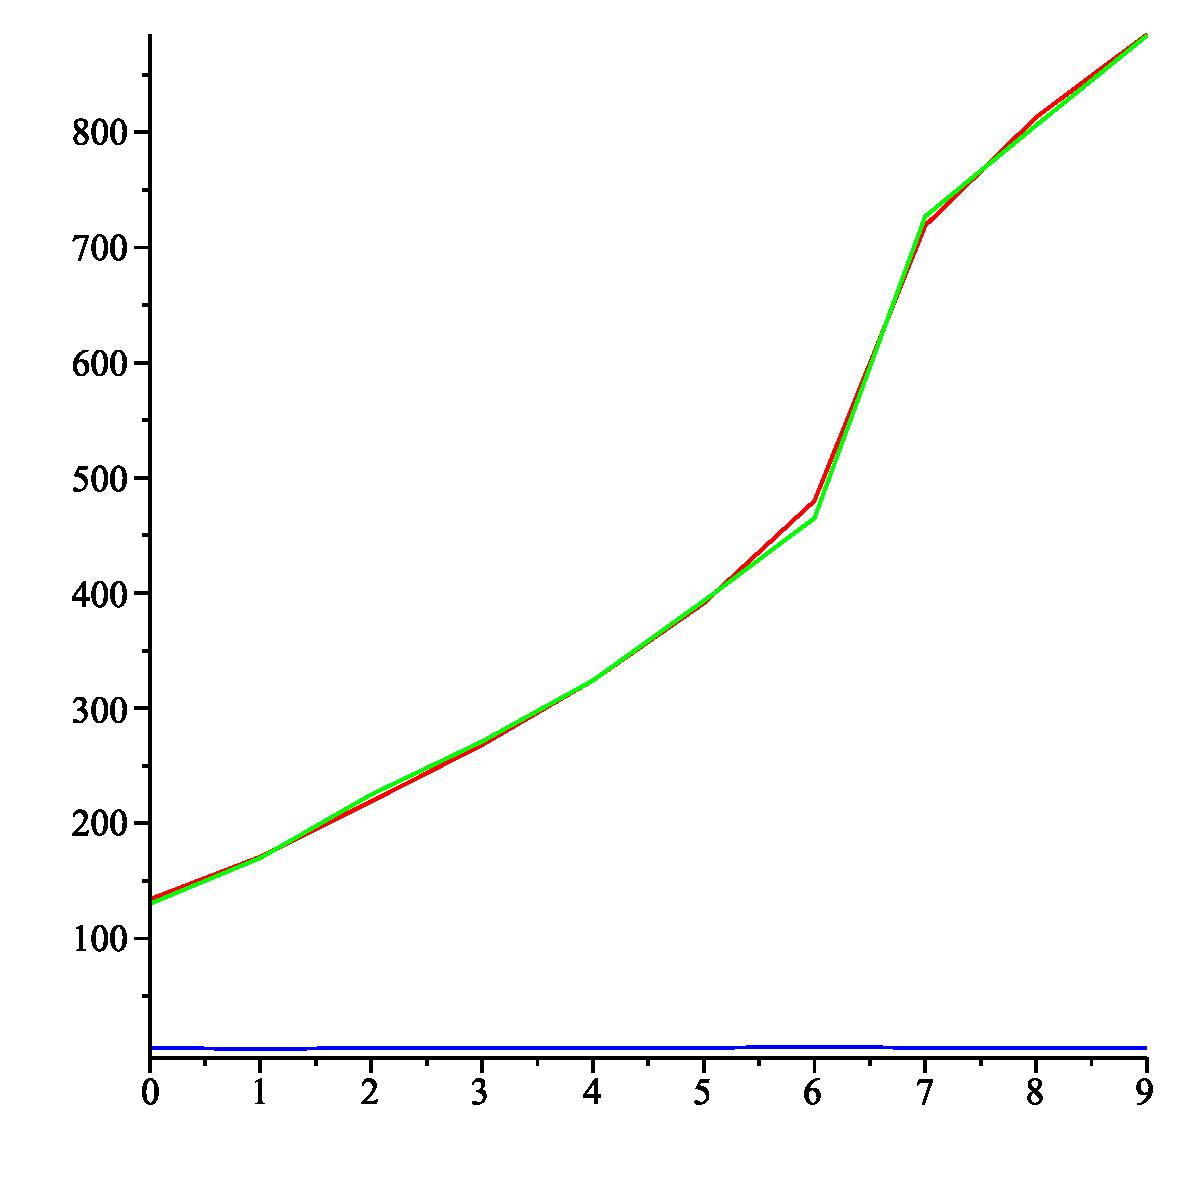
\includegraphics[width=1\textwidth]{alfp_graph.eps}

The red line executions times for the differential algorithm, the blue line is our implementation, and the green line is the BDD based algorithm. The values can be seen in appendix 7.6.

As the graph shows, the time for our implementation is very close to constant in this test, while the time for both algorithms rises. Something strange happens between execution 7 and 8, as the time jumps with just over 200 ms. It was also about that point where it took up to 10 executions before the time were as low as those in the graph. Instead, the execution time would be somewhere from 1000 ms to 4000 ms, and usually about 1400 ms. Perhaps the size of storing the calculations which needed to be done on the clauses, became higher than what the kernel wanted to cache, and therefore it had to load in the rest of the calculations before it could continue. Perhaps it had to rehash everything because the number of clauses where higher than there were space for. No matter what the reason is, the use of the succinct solver is still the slowest solution to use.

\subsection{Comparison}

The Succinct Solver gave surprisingly slow results. To give a worst-case for ourselves
to give a favorable comparison for the Succinct Solver, we generate some programs with
multiple loops, which would cause our worklist to reiterate all over again. The programs
consists of a loop with a recursive definition of itself. In the innermost loop, the statement
is a skip.

\begin{figure}
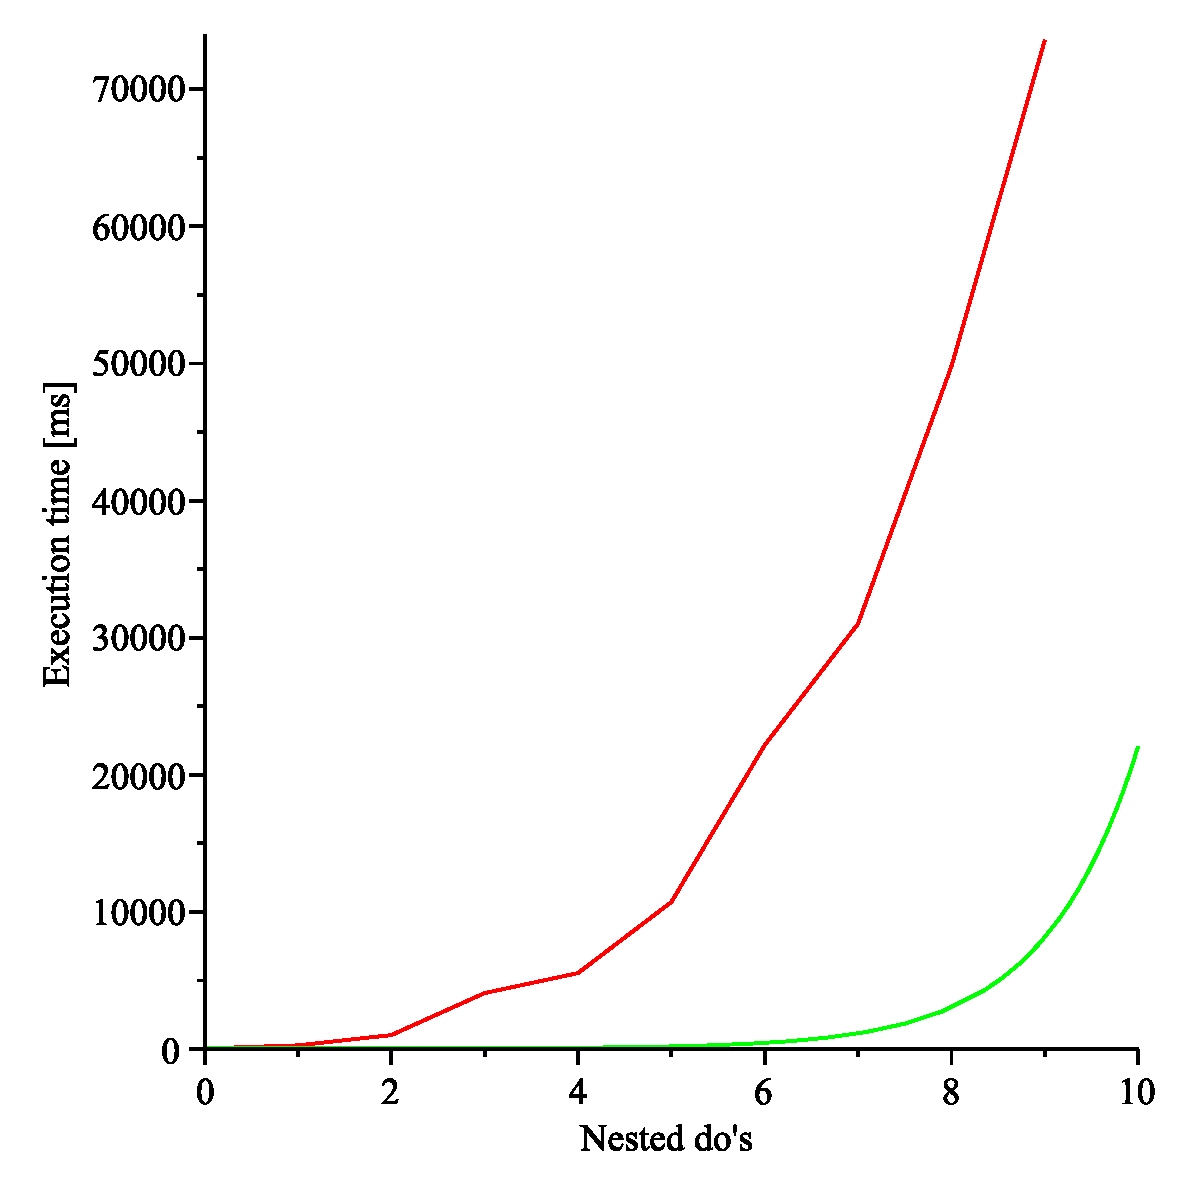
\includegraphics[width=1\textwidth]{alfp_nested_do_graph.eps}
\caption{Red is Succinct Solver, green is the function $e^x$, and the horizontal blue line is our worklist.}
\end{figure}

As can be seen on figure 4.1, the conclusion is that it this does not help. The result is worse. Another possible cause that have
been considered is that the internal representation of the program data structure uses
multiple temporary variables, which results in more variables when converting to the Succinct Solver
input form. To see if this will give the Succinct Solver an advantage (or
at least better efficiency), programs are generated without any temporary
variables. The basis of these programs are group 15's example program group15\_1.module.
We remove the if-statements, and take out the 3*n first statements, testing with n starting
from 1 and going forward, and used that to construct each program. This produces no temporary
variables. And the results is shown on figure 4.2.

\begin{figure}
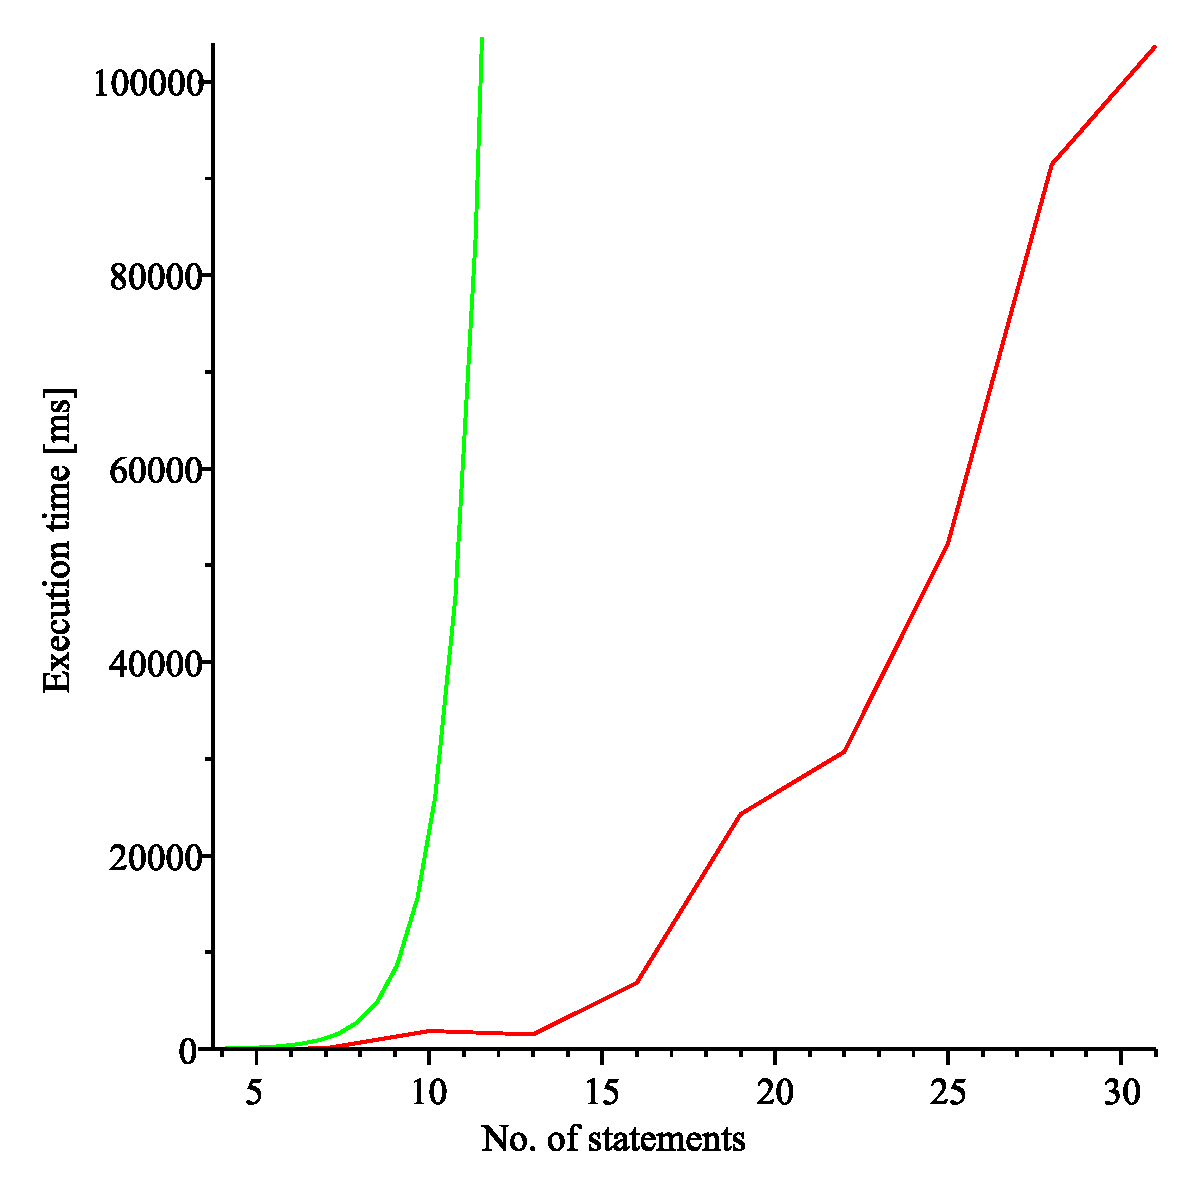
\includegraphics[width=1\textwidth]{alfp_mod15_graph.eps}
\caption{Red is Succinct Solver, green is the function $e^x$, and the horizontal blue line is our worklist.}
\end{figure}

It is shown that Succinct Solver does considerably better, but still considerably worse
than the worklist. This indicates that the temporary variables generated worsens the
efficiency considerably, but even without these temporary variables, the efficiency
is still much worse.

Finally, due to the temporary variables, comparing the running time of analyses of non-trivial programs
is difficult, since it seems to have a considerable impact on the running time, as seen above.
To do this, the temporary variables should either be removed, or they should be folded when
outputting the Succinct Solver input.



\chapter{Evaluation}


In the project, a program analysis module has been implemented.
Below, the different parts will be discussed.

\paragraph{Analyses:}
The 3 required analyses have been implemented in the project,
and the theory behind them have been described. Of note is that
SLVA has been implemented, to provide a more precise analysis
and a more effective Dead Code Elimination. We believe that SLVA
is important for the performance of DCE, since it frequently gives
a much more precise transformation. An example is given where LVA
keeps resurrecting faint variables, which should be removed, while
SLVA marks them as dead.

The constant propagation
has furthermore been given support for branch killing, which is also
quite useful. Killing branches can occur quite often in programs, for
instance in the case that a branch containing debug-code/test code
is killed because its condition is set to false (for instance through
a global constant).

The analyses have been tested by hand, but not through automated tests.
Besides this testing, they have been tested indirectly through the
transformations, because the transformations rely on the analyses being
correct.

Given the testing of the analyses and the performance of the transformations,
it is estimated that the analyses have been defined and implemented correctly.
Given the time frame and scope of the project, this is deemed sufficient
regarding the correctness of the analyses.

\paragraph{Transformations:}
The 3 required transformations, Program Slicing, Dead Code Elimination
and Constant Propagation, have been fully implemented.

Program Slicing is deemed to being implemented correctly, based on the
tests performed. The definition of PS can vary a lot, but it is deemed
that the definition in this project is both useful and somewhat simple.
This is confirmed by the implementation of PS. The definitionen not only
shows the relevant parts, but also preserves a runnable program, which
may be useful. Some other groups' definition of PS varies from this definition,
some ignoring control flow and focusing solely on the RD.
We believe that this definition gives a more usable PS, but this may depend
on the purpose of the PS. The purposes can include debugging for the
programmer, which suits this definition well.

The Dead Code Elimination is deemed to be very useful internally in regards
to cleaning up from other transformations. While it is rare for programmers
not to use variables, transformations frequently do not clean up after themselves,
including PS and CF. Another use for DCE is marking code for the programmer
that is dead, which although rare may indicate bugs.

The Constant Folding is deemed to be quite useful, especially given its
branch killing. As mentioned in the evaluation of the analyses,
branch killing can remove considerable parts of the code that ends up
in the final result, but can also increase the speed of the analyses and
transformations in general, because dead code is not investigated with
branch killing.

It is deemed that all the transformations perform well, and that they
have been tested well with both general programs and special case programs.

\paragraph{Worklist:}
The worklist implemented has focused less on generalisation, and more
on efficiency. In this regard, the worklist has performed admirably.
As seen in the test regarding the Succint Solver, it outperforms
the other methods, especially when the problem instances scales.

This comes at a price in generality. However, it is deemed that
this price is acceptable for multiple reasons: it shows that a worklist
implemented for specific problem instances can severely outperform
general implementations; and it gives a much better performance.

\paragraph{Testing:}

The testing is based on regression-testing. This means that the precise expected
output is written by the tester, and the test then succeeds only if the resulting
output is exactly the same as the expected output. This may result in false negatives:
results that are correct but not the same as the expected will be registered as negatives.
While this is not optimal, it is considered acceptable. Partly since implementing tests other
than regression tests is outside the scope of the project, and partly since the current
transformations implemented produce the same output if they are correct.



\chapter{Conclusion}


In this project, a program analysis module have been
designed, implemented and tested. A theoretical background
have been given for the analyses, and the Succinct Solver
has been tested against the worklist in the project.

\paragraph{Analyses:}

All the required assignments regarding analyses have been performed.

The analyses have been given a theoretical background,
and is deemed to be defined and implemented correctly,
given the testing and the performance of the transformations.
Of note is the implementation of Strongly Live Variable Analysis,
giving a considerably better performance than the simpler Live Variable Analysis,
and the Constant Propagation branch killing, enabling removal of dead code based on branches.

Both SLVA and CP branch killing is recommended, since the authors
believe that their increased performance outweights the required
definition and work.

\paragraph{Transformations:}

All the required assignments regarding transformations have been performed.
The transformations have been defined, designed, implemented and tested.

The Program Slicing has been examined thoroughly, and given a definition which should
make the PS useful for debugging as well as other purposes. It has
been compared with other groups, and is considered to have performed
well, as well as following the definition given. The given definition of PS has not
been used in real life, and can therefore not be recommended at the given point in time.
We recommend investigating the use of PS more, possibly test PS, to decide which
definition of PS is useful and in which cases.

The Dead Code Elimination performs well, and benefits well from the SLVA. It has
been deemed to be useful to clean up dead code from other transformations,
and could be used to indicate dead code for the programmer. LVA is not guaranteed to
perform as well as SLVA, even through repeated runs. For projects
implementing DCE, SLVA is therefore strongly recommended.

The Constant Folding performs well, especially given the branch killing. As argued,
dead branches occur in both programmers code and internally after transformations,
which makes branch killing especially useful. Not only does this have the potential
to make the analyses more precise, it can also decrease the program size that have
to be considered. Based on this, we recommended Constant Folding.

\paragraph{Worklist:}
As seen in the comparsion with the Succinct Solver, the worklist performs admirably.
For the same problem instances, the efficiency difference is quite large, and the
results are the same. Based on this, it is our recommendation that whenever a
general solution vs. a performance-tuned solution regarding worklists is considered,
the performance of the general solution must be carefully evaluated. If it does not
fulfill the needs for efficiency, it may be fruitful to find/implement a more
specific solution.

The main disadvantage is the lack of generality. This means that this implementation
may have less uses without adaptation. However, the worklist is both useful and can
be used as a benchmark between general solutions and more specific solutions,
which may be useful given that GCL is a somewhat simple language.

\paragraph{General conclusion:}
It is estimated that the project is successful. All assignments have
been completed, and more parts than required in the assignment have been added,
including branch killing.



\chapter{Appendix}

\section{Abbreviations and acronyms}

This section contains a list of abbreviations and acronyms used in
the report.

\begin{itemize}
\item CP(A) - Constant Propagation (Analysis)
\item GCC - GNU Compiler Collection (or GNU C Compiler)
\item GCL - Guarded Command Language
\item IR - Intermediate (or Internal) Representation
\item LV(A) - Live Variable (Analysis)
\item RD(A) - Reaching Definitions (Analysis)
\item SLV(A) - Strongly Live Variable (Analysis)
\end{itemize}

\section{Test results}

This section will contain various test results, which should not be in the main sections of this report.

\subsection{Succinct solver, test 1}
\subsubsection{Analysis output}
\begin{lstlisting}
Starting analysis
Finished analysis, time: 15ms.
// Printing exit evaluation
module chain_test_1:
read x;       //ID: 4d47c5fc, Analysis: [x = 4d47c5fc; y = 0], is killed: false
read y;       //ID: 4e3eca90, Analysis: [x = 4d47c5fc; y = 4e3eca90], is killed: false
x := 1;       //ID: 19c1ea29, Analysis: [x = 19c1ea29; y = 4e3eca90], is killed: false
y := (x+2);       //ID: 4413ee, Analysis: [x = 19c1ea29; y = 4413ee], is killed: false
write (y)       //ID: 3597a37c, Analysis: [x = 19c1ea29; y = 4413ee], is killed: false
end
\end{lstlisting}
\subsubsection{Clauses}
var(x) \& var(y) \& 
label(0) \& label(19c1ea29) \& label(3597a37c) \& label(4413ee) \& label(4d47c5fc) \& label(4e3eca90) \& 
flow(4e3eca90,19c1ea29) \& flow(4d47c5fc,4e3eca90) \& flow(4413ee,3597a37c) \& flow(19c1ea29,4413ee) \& flow(0,4d47c5fc) \& 
(A lab. label(lab) $=>$ kill(4e3eca90,y,lab)) \& (A lab. label(lab) $=>$ kill(4413ee,y,lab)) \& (A lab. label(lab) $=>$ kill(4d47c5fc,x,lab)) \& (A lab. label(lab) $=>$ kill(19c1ea29,x,lab)) \& 
gen(4e3eca90,y,4e3eca90) \& gen(4413ee,y,4413ee) \& gen(4d47c5fc,x,4d47c5fc) \& gen(19c1ea29,x,19c1ea29) \& 
(A lab. A x. A d. var(x) \& label(d) \& (RDentry(lab,x,d) \& ! kill(lab,x,d)) $|$ gen(lab,x,d) $=>$ RDexit(lab,x,d)) \& 
(A lab1. A lab2. A x. A d. flow(lab1,lab2) \& RDexit(lab1,x,d) $=>$ RDentry(lab2,x,d)) \& 
(A x. var(x) $=>$ RDentry(4d47c5fc,x,0))
\subsubsection{Conclusion}
Equal

\subsection{Succinct solver, test 2}
\subsubsection{Analysis output}
\begin{lstlisting}
Starting analysis
Finished analysis, time: 4ms.
// Printing exit evaluation
module chain_test_2:
read x;       //ID: 23174b07, Analysis: [x = 23174b07; y = 0], is killed: false
read y;       //ID: 7c64dc11, Analysis: [x = 23174b07; y = 7c64dc11], is killed: false
y := (y+x);       //ID: 4413ee, Analysis: [x = 23174b07; y = 4413ee], is killed: false
x := (x+y);       //ID: 75786e64, Analysis: [x = 75786e64; y = 4413ee], is killed: false
do
   (x<y) ->       //ID: 6100ab23, Analysis: [x = 558385e3, 75786e64; y = 4413ee, 742808b3], is killed: false
      x := (x+1)       //ID: 558385e3, Analysis: [x = 558385e3; y = 4413ee, 742808b3], is killed: false
   [] (y<x) ->       //ID: 72e3b895, Analysis: [x = 558385e3, 75786e64; y = 4413ee, 742808b3], is killed: false
      y := (y+1)       //ID: 742808b3, Analysis: [x = 558385e3, 75786e64; y = 742808b3], is killed: false
od;       //ID: 70922804, Analysis: [x = 558385e3, 75786e64; y = 4413ee, 742808b3], is killed: false
write (y);       //ID: 58cf40f5, Analysis: [x = 558385e3, 75786e64; y = 4413ee, 742808b3], is killed: false
write (x)       //ID: eb1c260, Analysis: [x = 558385e3, 75786e64; y = 4413ee, 742808b3], is killed: false
end
\end{lstlisting}
\subsubsection{Clauses}
var(Temp5) \& var(Temp3) \& var(x) \& var(y) \& 
label(0) \& label(23174b07) \& label(4413ee) \& label(558385e3) \& label(58cf40f5) \& label(6100ab23) \& label(70922804) \& label(72e3b895) \& label(742808b3) \& label(75786e64) \& label(7c64dc11) \& label(eb1c260) \& 
flow(58cf40f5,eb1c260) \& flow(742808b3,70922804) \& flow(72e3b895,742808b3) \& flow(70535b58,72e3b895) \& flow(75786e64,70922804) \& flow(70922804,70535b58) \& flow(70922804,58cf40f5) \& flow(558385e3,70922804) \& flow(6100ab23,558385e3) \& flow(70922804,2dcb25f1) \& flow(4413ee,75786e64) \& flow(2dcb25f1,6100ab23) \& flow(7c64dc11,4413ee) \& flow(23174b07,7c64dc11) \& flow(0,23174b07) \& 
(A lab. label(lab) $=>$ kill(7c64dc11,y,lab)) \& (A lab. label(lab) $=>$ kill(742808b3,y,lab)) \& (A lab. label(lab) $=>$ kill(75786e64,x,lab)) \& (A lab. label(lab) $=>$ kill(72e3b895,Temp5,lab)) \& (A lab. label(lab) $=>$ kill(558385e3,x,lab)) \& (A lab. label(lab) $=>$ kill(6100ab23,Temp3,lab)) \& (A lab. label(lab) $=>$ kill(4413ee,y,lab)) \& (A lab. label(lab) $=>$ kill(23174b07,x,lab)) \& 
gen(7c64dc11,y,7c64dc11) \& gen(742808b3,y,742808b3) \& gen(75786e64,x,75786e64) \& gen(72e3b895,Temp5,72e3b895) \& gen(558385e3,x,558385e3) \& gen(6100ab23,Temp3,6100ab23) \& gen(4413ee,y,4413ee) \& gen(23174b07,x,23174b07) \& 
(A lab. A x. A d. var(x) \& label(d) \& (RDentry(lab,x,d) \& ! kill(lab,x,d)) $|$ gen(lab,x,d) $=>$ RDexit(lab,x,d)) \& 
(A lab1. A lab2. A x. A d. flow(lab1,lab2) \& RDexit(lab1,x,d) $=>$ RDentry(lab2,x,d)) \& 
(A x. var(x) $=>$ RDentry(23174b07,x,0))
\subsubsection{Conclusion}
Equal, the value of temporary variables is not interesting (and therefore not printed), since it is only going to be used in the statement right after it was created (3-address rule).

\subsection{Succinct solver, test 3}
\subsubsection{Analysis output}
\begin{lstlisting}
Starting analysis
Finished analysis, time: 4ms.
// Printing exit evaluation
module chain_test_3:
read x;       //ID: 4d47c5fc, Analysis: [x = 4d47c5fc; y = 0], is killed: false
read y;       //ID: 4e3eca90, Analysis: [x = 4d47c5fc; y = 4e3eca90], is killed: false
y := (y+x);       //ID: 9f436f5, Analysis: [x = 4d47c5fc; y = 9f436f5], is killed: false
x := (x+y);       //ID: 4413ee, Analysis: [x = 4413ee; y = 9f436f5], is killed: false
if
   (x<y) ->       //ID: 19908ca1, Analysis: [x = 4413ee; y = 9f436f5], is killed: false
      x := (x+1)       //ID: 3f7fa65e, Analysis: [x = 3f7fa65e; y = 9f436f5], is killed: false
   [] (y<x) ->       //ID: 6100ab23, Analysis: [x = 4413ee; y = 9f436f5], is killed: false
      y := (y+1)       //ID: 2dcb25f1, Analysis: [x = 4413ee; y = 2dcb25f1], is killed: false
fi;       //ID: 70535b58, Analysis: [x = 4413ee, 3f7fa65e; y = 9f436f5, 2dcb25f1], is killed: false
write (y);       //ID: b815859, Analysis: [x = 4413ee, 3f7fa65e; y = 9f436f5, 2dcb25f1], is killed: false
write (x)       //ID: 58cf40f5, Analysis: [x = 4413ee, 3f7fa65e; y = 9f436f5, 2dcb25f1], is killed: false
end
\end{lstlisting}
\subsubsection{Clauses}
var(Temp5) \& var(Temp3) \& var(x) \& var(y) \& 
label(0) \& label(19908ca1) \& label(2dcb25f1) \& label(3f7fa65e) \& label(4413ee) \& label(4d47c5fc) \& label(4e3eca90) \& label(58cf40f5) \& label(6100ab23) \& label(70535b58) \& label(9f436f5) \& label(b815859) \& 
flow(b815859,58cf40f5) \& flow(3f7fa65e,b815859) \& flow(2dcb25f1,b815859) \& flow(742808b3,6100ab23) \& flow(70535b58,742808b3) \& flow(70535b58,558385e3) \& flow(9f436f5,4413ee) \& flow(6100ab23,2dcb25f1) \& flow(558385e3,19908ca1) \& flow(4e3eca90,9f436f5) \& flow(4413ee,70535b58) \& flow(4d47c5fc,4e3eca90) \& flow(19908ca1,3f7fa65e) \& flow(0,4d47c5fc) \& 
(A lab. label(lab) $=>$ kill(9f436f5,y,lab)) \& (A lab. label(lab) $=>$ kill(6100ab23,Temp5,lab)) \& (A lab. label(lab) $=>$ kill(4e3eca90,y,lab)) \& (A lab. label(lab) $=>$ kill(2dcb25f1,y,lab)) \& (A lab. label(lab) $=>$ kill(4d47c5fc,x,lab)) \& (A lab. label(lab) $=>$ kill(4413ee,x,lab)) \& (A lab. label(lab) $=>$ kill(3f7fa65e,x,lab)) \& (A lab. label(lab) $=>$ kill(19908ca1,Temp3,lab)) \& 
gen(9f436f5,y,9f436f5) \& gen(6100ab23,Temp5,6100ab23) \& gen(4e3eca90,y,4e3eca90) \& gen(2dcb25f1,y,2dcb25f1) \& gen(4d47c5fc,x,4d47c5fc) \& gen(4413ee,x,4413ee) \& gen(3f7fa65e,x,3f7fa65e) \& gen(19908ca1,Temp3,19908ca1) \& 
(A lab. A x. A d. var(x) \& label(d) \& (RDentry(lab,x,d) \& ! kill(lab,x,d)) $|$ gen(lab,x,d) $=>$ RDexit(lab,x,d)) \& 
(A lab1. A lab2. A x. A d. flow(lab1,lab2) \& RDexit(lab1,x,d) $=>$ RDentry(lab2,x,d)) \& 
(A x. var(x) $=>$ RDentry(4d47c5fc,x,0))
\subsubsection{Conclusion}
Equal, the value of temporary variables is not interesting (and therefore not printed), since it is only going to be used in the statement right after it was created (3-address rule).

\subsection{Succinct solver, test 4}
\subsubsection{Analysis output}
\begin{lstlisting}
Starting analysis
Finished analysis, time: 5ms.
// Printing exit evaluation
module chain_test_4:
read x;       //ID: 4d47c5fc, Analysis: [x = 4d47c5fc; y = 0], is killed: false
read y;       //ID: 4e3eca90, Analysis: [x = 4d47c5fc; y = 4e3eca90], is killed: false
y := (y+x);       //ID: 9f436f5, Analysis: [x = 4d47c5fc; y = 9f436f5], is killed: false
x := (x+y);       //ID: 4413ee, Analysis: [x = 4413ee; y = 9f436f5], is killed: false
if
   (x<y) ->       //ID: 7e0df503, Analysis: [x = 4413ee; y = 9f436f5], is killed: false
      x := (x+1)       //ID: 3f7fa65e, Analysis: [x = 3f7fa65e; y = 9f436f5], is killed: false
   [] (y<x) ->       //ID: 4650d89c, Analysis: [x = 4413ee; y = 9f436f5], is killed: false
      do
         (y<x) ->       //ID: 78b5f53a, Analysis: [x = 4413ee, b815859; y = 9f436f5, 70535b58], is killed: false
            y := (y+1)       //ID: 70535b58, Analysis: [x = 4413ee, b815859; y = 70535b58], is killed: false
         [] (y>x) ->       //ID: 71f6f0bf, Analysis: [x = 4413ee, b815859; y = 9f436f5, 70535b58], is killed: false
            x := (x+1)       //ID: b815859, Analysis: [x = b815859; y = 9f436f5, 70535b58], is killed: false
      od       //ID: eb1c260, Analysis: [x = 4413ee, b815859; y = 9f436f5, 70535b58], is killed: false
fi;       //ID: 19908ca1, Analysis: [x = 4413ee, b815859, 3f7fa65e; y = 9f436f5, 70535b58], is killed: false
write (y);       //ID: 72e3b895, Analysis: [x = 4413ee, b815859, 3f7fa65e; y = 9f436f5, 70535b58], is killed: false
write (x)       //ID: 446b7920, Analysis: [x = 4413ee, b815859, 3f7fa65e; y = 9f436f5, 70535b58], is killed: false
end
\end{lstlisting}
\subsubsection{Clauses}
var(Temp8) \& var(Temp6) \& var(Temp5) \& var(Temp3) \& var(x) \& var(y) \& 
label(0) \& label(19908ca1) \& label(3f7fa65e) \& label(4413ee) \& label(446b7920) \& label(4650d89c) \& label(4d47c5fc) \& label(4e3eca90) \& label(70535b58) \& label(71f6f0bf) \& label(72e3b895) \& label(78b5f53a) \& label(7e0df503) \& label(9f436f5) \& label(b815859) \& label(eb1c260) \& 
flow(eb1c260,72e3b895) \& flow(b815859,eb1c260) \& flow(71f6f0bf,b815859) \& flow(70535b58,eb1c260) \& flow(70922804,78b5f53a) \& flow(3f7fa65e,72e3b895) \& flow(58cf40f5,71f6f0bf) \& flow(eb1c260,70922804) \& flow(eb1c260,58cf40f5) \& flow(78b5f53a,70535b58) \& flow(72e3b895,446b7920) \& flow(4650d89c,eb1c260) \& flow(558385e3,7e0df503) \& flow(9f436f5,4413ee) \& flow(7e0df503,3f7fa65e) \& flow(4e3eca90,9f436f5) \& flow(19908ca1,558385e3) \& flow(4d47c5fc,4e3eca90) \& flow(38503429,4650d89c) \& flow(19908ca1,38503429) \& flow(4413ee,19908ca1) \& flow(0,4d47c5fc) \& 
(A lab. label(lab) $=>$ kill(b815859,x,lab)) \& (A lab. label(lab) $=>$ kill(9f436f5,y,lab)) \& (A lab. label(lab) $=>$ kill(70535b58,y,lab)) \& (A lab. label(lab) $=>$ kill(7e0df503,Temp3,lab)) \& (A lab. label(lab) $=>$ kill(78b5f53a,Temp6,lab)) \& (A lab. label(lab) $=>$ kill(71f6f0bf,Temp8,lab)) \& (A lab. label(lab) $=>$ kill(4e3eca90,y,lab)) \& (A lab. label(lab) $=>$ kill(4d47c5fc,x,lab)) \& (A lab. label(lab) $=>$ kill(4650d89c,Temp5,lab)) \& (A lab. label(lab) $=>$ kill(4413ee,x,lab)) \& (A lab. label(lab) $=>$ kill(3f7fa65e,x,lab)) \& 
gen(b815859,x,b815859) \& gen(9f436f5,y,9f436f5) \& gen(70535b58,y,70535b58) \& gen(7e0df503,Temp3,7e0df503) \& gen(78b5f53a,Temp6,78b5f53a) \& gen(71f6f0bf,Temp8,71f6f0bf) \& gen(4e3eca90,y,4e3eca90) \& gen(4d47c5fc,x,4d47c5fc) \& gen(4650d89c,Temp5,4650d89c) \& gen(4413ee,x,4413ee) \& gen(3f7fa65e,x,3f7fa65e) \& 
(A lab. A x. A d. var(x) \& label(d) \& (RDentry(lab,x,d) \& ! kill(lab,x,d)) $|$ gen(lab,x,d) $=>$ RDexit(lab,x,d)) \& 
(A lab1. A lab2. A x. A d. flow(lab1,lab2) \& RDexit(lab1,x,d) $=>$ RDentry(lab2,x,d)) \& 
(A x. var(x) $=>$ RDentry(4d47c5fc,x,0))
\subsubsection{Conclusion}
Equal, the value of temporary variables is not interesting (and therefore not printed), since it is only going to be used in the statement right after it was created (3-address rule).

\subsection{Succinct solver, test 5}
\subsubsection{Analysis output}
\begin{lstlisting}
Starting analysis
Finished analysis, time: 5ms.
// Printing exit evaluation
module chain_test_5:
read x;       //ID: 4d47c5fc, Analysis: [x = 4d47c5fc; y = 0], is killed: false
read y;       //ID: 4e3eca90, Analysis: [x = 4d47c5fc; y = 4e3eca90], is killed: false
y := (y+x);       //ID: 9f436f5, Analysis: [x = 4d47c5fc; y = 9f436f5], is killed: false
x := (x+y);       //ID: 4413ee, Analysis: [x = 4413ee; y = 9f436f5], is killed: false
do
   (x<y) ->       //ID: 4650d89c, Analysis: [x = 4413ee, 3f7fa65e, 70922804; y = 9f436f5, 58cf40f5], is killed: false
      x := (x+1)       //ID: 3f7fa65e, Analysis: [x = 3f7fa65e; y = 9f436f5, 58cf40f5], is killed: false
   [] (y<x) ->       //ID: 65bd0dd4, Analysis: [x = 4413ee, 3f7fa65e, 70922804; y = 9f436f5, 58cf40f5], is killed: false
      if
         (y>x) ->       //ID: 71f6f0bf, Analysis: [x = 4413ee, 3f7fa65e, 70922804; y = 9f436f5, 58cf40f5], is killed: false
            x := (x+1)       //ID: 70922804, Analysis: [x = 70922804; y = 9f436f5, 58cf40f5], is killed: false
         [] (y<=x) ->       //ID: b37c60d, Analysis: [x = 4413ee, 3f7fa65e, 70922804; y = 9f436f5, 58cf40f5], is killed: false
            y := (y+1)       //ID: 58cf40f5, Analysis: [x = 4413ee, 3f7fa65e, 70922804; y = 58cf40f5], is killed: false
      fi       //ID: 38503429, Analysis: [x = 4413ee, 3f7fa65e, 70922804; y = 9f436f5, 58cf40f5], is killed: false
od;       //ID: 6100ab23, Analysis: [x = 4413ee, 3f7fa65e, 70922804; y = 9f436f5, 58cf40f5], is killed: false
write (y);       //ID: 446b7920, Analysis: [x = 4413ee, 3f7fa65e, 70922804; y = 9f436f5, 58cf40f5], is killed: false
write (x)       //ID: 6bdd46f7, Analysis: [x = 4413ee, 3f7fa65e, 70922804; y = 9f436f5, 58cf40f5], is killed: false
end
\end{lstlisting}
\subsubsection{Clauses}
var(Temp8) \& var(Temp6) \& var(Temp5) \& var(Temp3) \& var(x) \& var(y) \& 
label(0) \& label(38503429) \& label(3f7fa65e) \& label(4413ee) \& label(446b7920) \& label(4650d89c) \& label(4d47c5fc) \& label(4e3eca90) \& label(58cf40f5) \& label(6100ab23) \& label(65bd0dd4) \& label(6bdd46f7) \& label(70922804) \& label(71f6f0bf) \& label(9f436f5) \& label(b37c60d) \& 
flow(eb1c260,b37c60d) \& flow(38503429,eb1c260) \& flow(b815859,71f6f0bf) \& flow(b37c60d,58cf40f5) \& flow(71f6f0bf,70922804) \& flow(70922804,6100ab23) \& flow(58cf40f5,6100ab23) \& flow(38503429,b815859) \& flow(65bd0dd4,38503429) \& flow(6100ab23,558385e3) \& flow(6100ab23,446b7920) \& flow(6100ab23,19908ca1) \& flow(558385e3,4650d89c) \& flow(9f436f5,4413ee) \& flow(4e3eca90,9f436f5) \& flow(446b7920,6bdd46f7) \& flow(19908ca1,65bd0dd4) \& flow(4413ee,6100ab23) \& flow(3f7fa65e,6100ab23) \& flow(4d47c5fc,4e3eca90) \& flow(4650d89c,3f7fa65e) \& flow(0,4d47c5fc) \& 
(A lab. label(lab) $=>$ kill(b37c60d,Temp8,lab)) \& (A lab. label(lab) $=>$ kill(9f436f5,y,lab)) \& (A lab. label(lab) $=>$ kill(58cf40f5,y,lab)) \& (A lab. label(lab) $=>$ kill(70922804,x,lab)) \& (A lab. label(lab) $=>$ kill(71f6f0bf,Temp6,lab)) \& (A lab. label(lab) $=>$ kill(65bd0dd4,Temp5,lab)) \& (A lab. label(lab) $=>$ kill(4e3eca90,y,lab)) \& (A lab. label(lab) $=>$ kill(4d47c5fc,x,lab)) \& (A lab. label(lab) $=>$ kill(3f7fa65e,x,lab)) \& (A lab. label(lab) $=>$ kill(4650d89c,Temp3,lab)) \& (A lab. label(lab) $=>$ kill(4413ee,x,lab)) \& 
gen(b37c60d,Temp8,b37c60d) \& gen(9f436f5,y,9f436f5) \& gen(58cf40f5,y,58cf40f5) \& gen(70922804,x,70922804) \& gen(71f6f0bf,Temp6,71f6f0bf) \& gen(65bd0dd4,Temp5,65bd0dd4) \& gen(4e3eca90,y,4e3eca90) \& gen(4d47c5fc,x,4d47c5fc) \& gen(3f7fa65e,x,3f7fa65e) \& gen(4650d89c,Temp3,4650d89c) \& gen(4413ee,x,4413ee) \& 
(A lab. A x. A d. var(x) \& label(d) \& (RDentry(lab,x,d) \& ! kill(lab,x,d)) $|$ gen(lab,x,d) $=>$ RDexit(lab,x,d)) \& 
(A lab1. A lab2. A x. A d. flow(lab1,lab2) \& RDexit(lab1,x,d) $=>$ RDentry(lab2,x,d)) \& 
(A x. var(x) $=>$ RDentry(4d47c5fc,x,0))
\subsubsection{Conclusion}
Equal, the value of temporary variables is not interesting (and therefore not printed), since it is only going to be used in the statement right after it was created (3-address rule).

\subsection{Succinct solver, test 6}
\subsubsection{Analysis output}
\begin{lstlisting}
Starting analysis
Finished analysis, time: 5ms.
// Printing exit evaluation
module chain_test_6:
read x;       //ID: 4d47c5fc, Analysis: [x = 4d47c5fc; y = 0], is killed: false
read y;       //ID: 4e3eca90, Analysis: [x = 4d47c5fc; y = 4e3eca90], is killed: false
y := (y+x);       //ID: 9f436f5, Analysis: [x = 4d47c5fc; y = 9f436f5], is killed: false
x := (x+y);       //ID: 4413ee, Analysis: [x = 4413ee; y = 9f436f5], is killed: false
if
   (x<y) ->       //ID: c5e3974, Analysis: [x = 4413ee; y = 9f436f5], is killed: false
      x := (x+1)       //ID: 3f7fa65e, Analysis: [x = 3f7fa65e; y = 9f436f5], is killed: false
   [] (y<x) ->       //ID: 7e0df503, Analysis: [x = 4413ee; y = 9f436f5], is killed: false
      if
         (y<x) ->       //ID: 5ed70d7a, Analysis: [x = 4413ee; y = 9f436f5], is killed: false
            y := (y+1)       //ID: 742808b3, Analysis: [x = 4413ee; y = 742808b3], is killed: false
         [] (y>x) ->       //ID: 78b5f53a, Analysis: [x = 4413ee; y = 9f436f5], is killed: false
            x := (x+1)       //ID: 70922804, Analysis: [x = 70922804; y = 9f436f5], is killed: false
      fi       //ID: 58cf40f5, Analysis: [x = 4413ee, 70922804; y = 9f436f5, 742808b3], is killed: false
fi;       //ID: 38503429, Analysis: [x = 4413ee, 3f7fa65e, 70922804; y = 9f436f5, 742808b3], is killed: false
write (y);       //ID: 6100ab23, Analysis: [x = 4413ee, 3f7fa65e, 70922804; y = 9f436f5, 742808b3], is killed: false
write (x)       //ID: 72e3b895, Analysis: [x = 4413ee, 3f7fa65e, 70922804; y = 9f436f5, 742808b3], is killed: false
end
\end{lstlisting}
\subsubsection{Clauses}
var(Temp8) \& var(Temp6) \& var(Temp5) \& var(Temp3) \& var(x) \& var(y) \& 
label(0) \& label(38503429) \& label(3f7fa65e) \& label(4413ee) \& label(4d47c5fc) \& label(4e3eca90) \& label(58cf40f5) \& label(5ed70d7a) \& label(6100ab23) \& label(70922804) \& label(72e3b895) \& label(742808b3) \& label(78b5f53a) \& label(7e0df503) \& label(9f436f5) \& label(c5e3974) \& 
flow(58cf40f5,b815859) \& flow(eb1c260,7e0df503) \& flow(b815859,78b5f53a) \& flow(6100ab23,72e3b895) \& flow(78b5f53a,70922804) \& flow(742808b3,6100ab23) \& flow(70922804,6100ab23) \& flow(5ed70d7a,742808b3) \& flow(70535b58,5ed70d7a) \& flow(58cf40f5,70535b58) \& flow(7e0df503,58cf40f5) \& flow(38503429,eb1c260) \& flow(c5e3974,3f7fa65e) \& flow(558385e3,c5e3974) \& flow(9f436f5,4413ee) \& flow(4e3eca90,9f436f5) \& flow(3f7fa65e,6100ab23) \& flow(38503429,558385e3) \& flow(4d47c5fc,4e3eca90) \& flow(4413ee,38503429) \& flow(0,4d47c5fc) \& 
(A lab. label(lab) $=>$ kill(c5e3974,Temp3,lab)) \& (A lab. label(lab) $=>$ kill(9f436f5,y,lab)) \& (A lab. label(lab) $=>$ kill(742808b3,y,lab)) \& (A lab. label(lab) $=>$ kill(70922804,x,lab)) \& (A lab. label(lab) $=>$ kill(7e0df503,Temp5,lab)) \& (A lab. label(lab) $=>$ kill(78b5f53a,Temp8,lab)) \& (A lab. label(lab) $=>$ kill(5ed70d7a,Temp6,lab)) \& (A lab. label(lab) $=>$ kill(4e3eca90,y,lab)) \& (A lab. label(lab) $=>$ kill(4d47c5fc,x,lab)) \& (A lab. label(lab) $=>$ kill(4413ee,x,lab)) \& (A lab. label(lab) $=>$ kill(3f7fa65e,x,lab)) \& 
gen(c5e3974,Temp3,c5e3974) \& gen(9f436f5,y,9f436f5) \& gen(742808b3,y,742808b3) \& gen(70922804,x,70922804) \& gen(7e0df503,Temp5,7e0df503) \& gen(78b5f53a,Temp8,78b5f53a) \& gen(5ed70d7a,Temp6,5ed70d7a) \& gen(4e3eca90,y,4e3eca90) \& gen(4d47c5fc,x,4d47c5fc) \& gen(4413ee,x,4413ee) \& gen(3f7fa65e,x,3f7fa65e) \& 
(A lab. A x. A d. var(x) \& label(d) \& (RDentry(lab,x,d) \& ! kill(lab,x,d)) $|$ gen(lab,x,d) $=>$ RDexit(lab,x,d)) \& 
(A lab1. A lab2. A x. A d. flow(lab1,lab2) \& RDexit(lab1,x,d) $=>$ RDentry(lab2,x,d)) \& 
(A x. var(x) $=>$ RDentry(4d47c5fc,x,0))
\subsubsection{Conclusion}
Equal, the value of temporary variables is not interesting (and therefore not printed), since it is only going to be used in the statement right after it was created (3-address rule).

\subsection{Succinct solver, test 7}
\subsubsection{Analysis output}
\begin{lstlisting}
Starting analysis
Finished analysis, time: 6ms.
// Printing exit evaluation
module chain_test_7:
read x;       //ID: 23174b07, Analysis: [x = 23174b07; y = 0], is killed: false
read y;       //ID: 7c64dc11, Analysis: [x = 23174b07; y = 7c64dc11], is killed: false
y := (y+x);       //ID: 4413ee, Analysis: [x = 23174b07; y = 4413ee], is killed: false
x := (x+y);       //ID: 75786e64, Analysis: [x = 75786e64; y = 4413ee], is killed: false
do
   (x<y) ->       //ID: 4650d89c, Analysis: [x = 558385e3, 70922804, 75786e64; y = 4413ee, 58cf40f5], is killed: false
      x := (x+1)       //ID: 558385e3, Analysis: [x = 558385e3; y = 4413ee, 58cf40f5], is killed: false
   [] (y<x) ->       //ID: 65bd0dd4, Analysis: [x = 558385e3, 70922804, 75786e64; y = 4413ee, 58cf40f5], is killed: false
      do
         (y>x) ->       //ID: 71f6f0bf, Analysis: [x = 558385e3, 70922804, 75786e64; y = 4413ee, 58cf40f5], is killed: false
            x := (x+1)       //ID: 70922804, Analysis: [x = 70922804; y = 4413ee, 58cf40f5], is killed: false
         [] (y<=x) ->       //ID: b37c60d, Analysis: [x = 558385e3, 70922804, 75786e64; y = 4413ee, 58cf40f5], is killed: false
            y := (y+1)       //ID: 58cf40f5, Analysis: [x = 558385e3, 70922804, 75786e64; y = 58cf40f5], is killed: false
      od       //ID: 38503429, Analysis: [x = 558385e3, 70922804, 75786e64; y = 4413ee, 58cf40f5], is killed: false
od;       //ID: 6100ab23, Analysis: [x = 558385e3, 70922804, 75786e64; y = 4413ee, 58cf40f5], is killed: false
write (y);       //ID: 446b7920, Analysis: [x = 558385e3, 70922804, 75786e64; y = 4413ee, 58cf40f5], is killed: false
write (x)       //ID: 6bdd46f7, Analysis: [x = 558385e3, 70922804, 75786e64; y = 4413ee, 58cf40f5], is killed: false
end
\end{lstlisting}
\subsubsection{Clauses}
var(Temp8) \& var(Temp6) \& var(Temp5) \& var(Temp3) \& var(x) \& var(y) \& 
label(0) \& label(23174b07) \& label(38503429) \& label(4413ee) \& label(446b7920) \& label(4650d89c) \& label(558385e3) \& label(58cf40f5) \& label(6100ab23) \& label(65bd0dd4) \& label(6bdd46f7) \& label(70922804) \& label(71f6f0bf) \& label(75786e64) \& label(7c64dc11) \& label(b37c60d) \& 
flow(eb1c260,b37c60d) \& flow(b37c60d,58cf40f5) \& flow(38503429,eb1c260) \& flow(b815859,71f6f0bf) \& flow(71f6f0bf,70922804) \& flow(446b7920,6bdd46f7) \& flow(38503429,b815859) \& flow(75786e64,6100ab23) \& flow(6100ab23,446b7920) \& flow(70922804,38503429) \& flow(65bd0dd4,38503429) \& flow(58cf40f5,38503429) \& flow(6100ab23,19908ca1) \& flow(558385e3,6100ab23) \& flow(4650d89c,558385e3) \& flow(6100ab23,2dcb25f1) \& flow(4413ee,75786e64) \& flow(38503429,6100ab23) \& flow(2dcb25f1,4650d89c) \& flow(7c64dc11,4413ee) \& flow(23174b07,7c64dc11) \& flow(19908ca1,65bd0dd4) \& flow(0,23174b07) \& 
(A lab. label(lab) $=>$ kill(b37c60d,Temp8,lab)) \& (A lab. label(lab) $=>$ kill(7c64dc11,y,lab)) \& (A lab. label(lab) $=>$ kill(58cf40f5,y,lab)) \& (A lab. label(lab) $=>$ kill(75786e64,x,lab)) \& (A lab. label(lab) $=>$ kill(70922804,x,lab)) \& (A lab. label(lab) $=>$ kill(71f6f0bf,Temp6,lab)) \& (A lab. label(lab) $=>$ kill(65bd0dd4,Temp5,lab)) \& (A lab. label(lab) $=>$ kill(558385e3,x,lab)) \& (A lab. label(lab) $=>$ kill(4650d89c,Temp3,lab)) \& (A lab. label(lab) $=>$ kill(4413ee,y,lab)) \& (A lab. label(lab) $=>$ kill(23174b07,x,lab)) \& 
gen(b37c60d,Temp8,b37c60d) \& gen(7c64dc11,y,7c64dc11) \& gen(58cf40f5,y,58cf40f5) \& gen(75786e64,x,75786e64) \& gen(70922804,x,70922804) \& gen(71f6f0bf,Temp6,71f6f0bf) \& gen(65bd0dd4,Temp5,65bd0dd4) \& gen(558385e3,x,558385e3) \& gen(4650d89c,Temp3,4650d89c) \& gen(4413ee,y,4413ee) \& gen(23174b07,x,23174b07) \& 
(A lab. A x. A d. var(x) \& label(d) \& (RDentry(lab,x,d) \& ! kill(lab,x,d)) $|$ gen(lab,x,d) $=>$ RDexit(lab,x,d)) \& 
(A lab1. A lab2. A x. A d. flow(lab1,lab2) \& RDexit(lab1,x,d) $=>$ RDentry(lab2,x,d)) \& 
(A x. var(x) $=>$ RDentry(23174b07,x,0))
\subsubsection{Conclusion}
Equal, the value of temporary variables is not interesting (and therefore not printed), since it is only going to be used in the statement right after it was created (3-address rule).

\subsection{Succinct solver, execution times}
\begin{center}
	\begin{tabular}{ | c | c | c | }
		\hline
		Ours [ms] & Differential algorithm [ms] & BDD based algorithm [ms] \\
		\hline
		\hline
		5 & 134 & 130 \\
		4 & 171 & 170 \\
		5 & 219 & 225 \\
		5 & 268 & 271 \\
		4 & 324 & 324 \\
		5 & 391 & 393 \\
		6 & 480 & 465 \\
		5 & 719 & 727 \\
		5 & 813 & 806 \\
		5 & 885 & 884 \\
		\hline
	\end{tabular}
\end{center}

\end{document}

